% This is based on the LLNCS.DEM the demonstration file of
% the LaTeX macro package from Springer-Verlag
% for Lecture Notes in Computer Science,
% version 2.4 for LaTeX2e as of 16.  April 2010
%
% See http://www.springer.com/computer/lncs/lncs+authors?SGWID=0-40209-0-0-0
% for the full guidelines.
%
\documentclass{llncs}
\usepackage{graphicx,psfrag,epsf}
\makeatletter
\newcommand{\figcaption}[1]{\def\@captype{figure}\caption{#1}}
\newcommand{\tblcaption}[1]{\def\@captype{table}\caption{#1}}
\makeatother

\begin{document}

%-----------------------------------------------------------------------------------------------------
%-----------------WARNING---------------
%I don't know how and why i can access to this document but you should protect it to avoid vandalizing, have a good day.  -AL
%-----------------------------------------------------------------------------------------------------

\title{A User Evaluation of Group in a Box Variants}
%
\titlerunning{GIB Evaluation}  % abbreviated title (for running head)
%                                     also used for the TOC unless
%                                     \toctitle is used
%
\author{Nozomi Aoyama, Yosuke Onoue, Kohei Arimoto, Yuki Ueno, Hiroaki Natsukawa, Koji Koyamada}
%
\authorrunning{Nozomi Aoyama} % abbreviated author list (for running head)
%
%%%% list of authors for the TOC (use if author list has to be modified)
\tocauthor{Nozomi Aoyama}
%
\institute{Kyoto University, Japan \\
\email{aoyama.nozomi.37x@st.kyoto-u.ac.jp}\\
\url{https://www.kyoto-u.ac.jp}}

\maketitle              % typeset the title of the contribution

\begin{abstract}
Group-In-a-Box (GIB) is a graph-drawing method designed for visualizing the group structure of graphs.
GIB enables to see group sizes and both inter- and intra-group structures simultaneously.
Several GIB variants have been proposed to realize each design goal.
However, their advantages and disadvantages from the perspective of human cognition have not been studied.
In this study, we conducted a user evaluation including eye-tracking analysis of 4 GIB variants to clarify them.
From the evaluation, we found some trade-offs among each method for type of user task.
The eye-tracking analysis gave us some clues to figure out the reasons why the results were caused.

\keywords{Group-in-a-box, user evaluation, eye tracking, graph drawing}
\end{abstract}

%
\section{Introduction}
%
In the area of graph drawing, numerous methods have been proposed and each aims a different visualization goal.
Real-world graph data such as social network or web graph often have a characteristic so-called complex networks \cite{newman10}.
One feature of complex networks is their community structure \cite{newman02,newman04}.
A network with community structure have some groups which consist of several nodes and have dense within-group edges and sparse between-group edges.
Additionally, real-world data often provide information on the groups to which the nodes belong.
In order to analyze real-world data, a effective visualization technique for understanding group structure is essential.

Group-In-a-Box (GIB) is a graph drawing method designed for visualizing the group structures in graphs \cite{rodri,chatu,onoue}.
GIB arranges all nodes in a group into a box with an area proportional to the number of nodes in the group.
Using a GIB layout enables the simultaneous visualization of group structures, between-group relationships, and the sizes of the groups in a graph.
There are several variations of GIB layout, and each of them has its advantage.
Although there are a few computational experiments \cite{chatu,onoue} to evaluate them, no one have done the evaluation of these GIB variants through user-study experiments to the best of our knowledge.
Some measures in networks such as the number of edge crossing are known to have an effect on readability of graph drawing \cite{becker,pur97,pur98,pca} but there are other elements related to readability in GIB visualizations, so user-study experiments is important.

In this study, we aim to find out which GIB variants is the most effective among .
We report on a evaluation of 4 GIB variants, ST-GIB, CD-GIB, FD-GIB and TR-GIB with 4 types of user tasks.
The tasks are designed based on the studies by Vehlow et al. \cite{survey} and Saket et al. \cite{saket} in order to see each layout's features from various perspectives.
We measured task accuracy and completion time at each task.
We also collect eye-tracking data of participants during the tasks.
Eye-tracking is useful for the analysis of tasks in this case a because we can get insights about why the layouts make difference in the result \cite{eyemethod}.
We analyze not only the accuracy and completion time of tasks but also eye-track data to reveal why a layout is better than the others.
% =======
% In the area of graph drawing, several methods have been proposed and each aims a different visualization goal. Real-world graph data such as social network or web graph often have a characteristic so-called complex networks \cite{newman10}. One feature of complex networks is their community structure \cite{newman02,newman04}. A network with community structure have some groups which consist of several nodes and have dense within-group edges and sparse between-group edges. Real-world data often provide information on the groups to which the nodes belong. In order to analyze real-world data, a effective visualization technique for understanding community structure is essential. 

% Group-In-a-Box (GIB) is a graph drawing method designed for visualizing the community structures in graphs \cite{rodri,chatu,onoue}. GIB arranges all nodes in a group into a box with an area proportional to the number of nodes in the group. Using a GIB layout enables the simultaneous visualization of group structures, between-group relationships, and the sizes of the groups in a graph. There are several GIB layout methods, and we expect that each of them has its merit. Although there are a few computational experiments \cite{chatu,onoue} to evaluate them, no one have done the evaluation of these GIB layouts through user-study experiments. Some measures in networks such as the number of edge crossing are known to have an effect on readability of graph drawing \cite{pur97,pur98,pca,becker} but there are other elements related to readability in GIB visualizations, so user-study experiments is important.

% In this study, We aim to find out which GIB layouts is the most effective among ST-GIB, CD-GIB, FD-GIB and TR-GIB. We report on two experiments for evaluation of 4 GIB layouts. The first one is computational, we implements more accurate and reliable calculation for comparison than the ever by using many and practical data.

% The second one is user study with 4 tasks and 4 layouts. The tasks are set based on \cite{survey,saket} in order to see each layout's features from various perspectives. We measured task accuracy and completion time at each task.  We also collect eye-tracking data of participants during experiments for evaluation. Eye-tracking is useful for the analysis of tasks in this case a because we can get insights about why the layouts make difference in the result \cite{eyemethod}. We analyze not only the accuracy and completion time of tasks but also eye-track data to reveal why a layout is better than the others.

%
\section{GIB Layouts}
%
In this section, we describe 4 GIB variants we evaluated, STGIB, CD-GIB, FD-GIB and TR-GIB.
The examples of layouts are show at Fig. \ref{GIB-examples}.

\begin{figure}[h]
  \begin{center}
    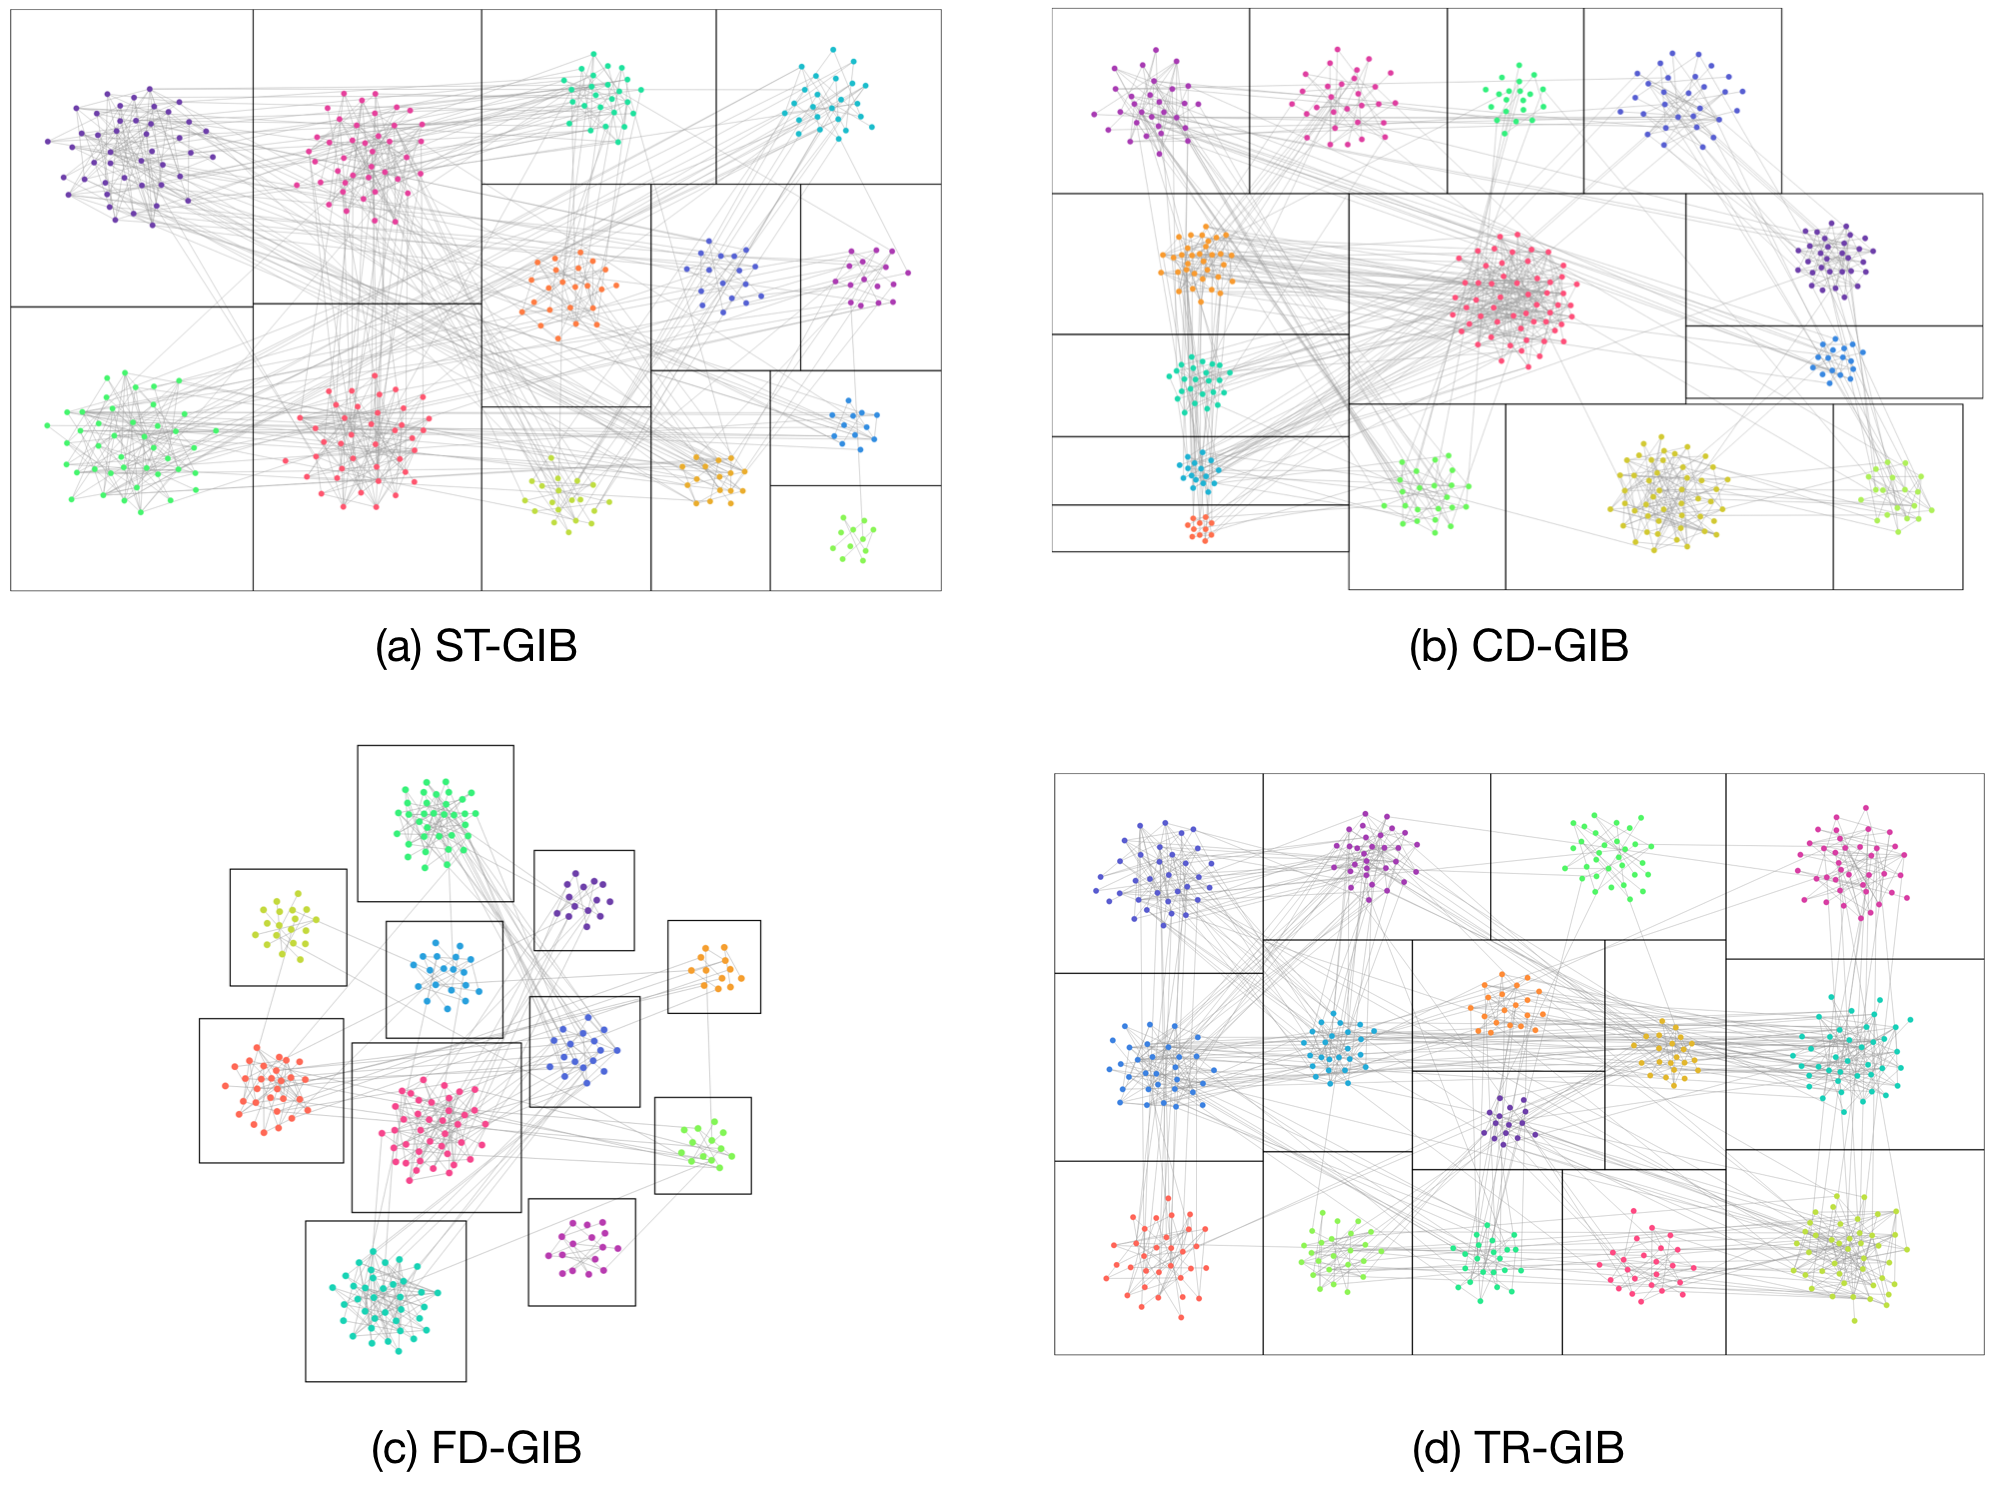
\includegraphics[width=1\textwidth]{example.png}
    \caption{Examples of GIB layouts}
    \label{GIB-examples}
  \end{center}
\end{figure}

\subsection{ST-GIB}
ST-GIB (Fig. \ref{GIB-examples} (a)), Squarified Treemap GIB, is a layout based on Bruls et al's Squarified Treemap \cite{bruls}, and proposed by Rodrigues et al \cite{rodri}.
Bruls' method is originally for treemaping, which is a visualization method that takes rectangular regions and numerical columns as inputs to divide a region into tiles with areas proportional to their values \cite{shn92}.

In the case of ST-GIB, their groups are taken as vertexes in treemaps and shown in the shape of tiles which have nodes that belong to its group in it.
The Treemap algorithm facilitates a space-filling arrangement with low box aspect ratios, which is important for analyzing the rectangle content \cite{bruls}.
ST-GIB layout, however, just uses a Squarified Treemap algorithm to layout group networks in rectangles, so it does not consider the information of relationships among nodes when the tiles are placed.
This problem causes link overlaps which have the greatest detrimental impact on understanding networks \cite{becker,pur97,pur98,pca}.
To arrange tiles along this method, we utilized a Python library Squarify (https://github.com/laserson/squarify), which employs Bruls' algorithm.


\subsection{CD-GIB}
CD-GIB, Croissant and Doughnut GIB, is proposed presented by Chaturvedi et al. \cite{chatu}, shown in Fig. \ref{GIB-examples} (b).
They developed this layout in order to improve ST-GIB for the sake of considering network information connecting a node to another of a different group. Concretely, they worked on arranging tiles based on G-degree and G-skewness.
A group's G-degree is defined as the number of other groups it is connected to, and G-skewness refers to the fraction of nodes present in the two most connected groups (groups with highest G-degree).
Then one layout are chosen from Croissant-GIB, Doughnut-GIB or ST-GIB according to the total number of groups, G, and G-skewness.
Chaturvedi define criteria to use 3 methods properly and we also use it.


The most connected box with the highest G-degree is placed close to center so that these method take into account links among groups, so we expect better readability than ST-GIB as a result of less edge crossings \cite{becker,pur97,pur98,pca}.
However, the aspect ratio of a box tend to be worse, which can affect the capability of being analyzed the rectangle content \cite{bruls}.


\subsection{FD-GIB}
The FD-GIB layout is also provided by Chaturvedi et al \cite{chatu}, Fig. \ref{GIB-examples} (c).
This is the approach for explicitly showing the inter-group relationships.
The group boxes are arranged using a force-directed layout run on the whole network, where the vertexes represent entire groups and the edges between them show the links between groups.
They then draw the group boxes on this initial layout centered at the group node’s position.
This layout can cause overlaps of groups, so the PRISM method are taken to remove laps, proposed by Gansner et al \cite{gansner}.
We eliminated all of overlaps using this method.

Chaturvedi use the the Harel–Koren FMS layout \cite{harel-koren} to arrange rectangles in FD-GIB, but we used the force simulation of D3.js (https://d3js.org/) because it was easy to avail and produced good results.
However, as Chaturvedi mentioned in \cite{chatu}, there are several good choice such as the high-dimensional embedding (HDE) approach of \cite{harel} or the algebraic multi-grid method (ACE) of \cite{koren}, according to experimental evaluations of several layout algorithms carried out by Hachul et al. \cite{hachul1,hachul2}.

This layout has a benefit of clearly showing the aggregate topology, but waste screen space more.
The area of each group must be smaller than the others, is is expected more difficult to see the relationships in a single group.
However this layout can maintain the box aspect ratio 1.0, so we expect participants can easily recognize the size difference between boxes.


\subsection{TR-GIB}
The TR-GIB is our previous works that minimize the weighed sum of distances between groups by reordering the sibling nodes in ST-GIB \cite{onoue}.
An example of this is shown in Fig. \ref{GIB-examples} (d).
This method looks like ST-GIB, but the tiles are reordered.
Treemaps such as ST-GIB has a structure of tree, so vertexes with same depth in it can be reordered.
This layout aims reducing the sum of distance of links, which leads to less edge crossing causing misunderstanding.
The coordinate of this layout can be gotten by reordering the coordinate of ST-GIB layout so that the proximity is minimized.
Specifically, the sum of the distances between two groups is weighted according to the number of edges between the two groups, and this sum is taken as the group proximity.

This layouts has the minimized group proximity, so the edges length is shortened which leads to less edge crossings than ST-GIB.
We expect that this layout have the both of the advantages of ST-GIB such as good aspect and screen efficiency, and the advantage of less edge overlaps.

%
\section{User Study Experiment}
%
We worked on the user study experiment with eye-track system.
We intended to reveal which layout were superior in some tasks through this study.
The layouts of GIB we compared were STGIB, CDGIB, FDGIB, and TRGIB.
In addition to accuracy and completion time of tasks, we also measured eye-tracking data to evaluate layouts quantitatively.
By using eye-track system, we can give elaborates discussion on the result \cite{eyemethod}.
We describe this experiment in this section.

\subsection{Task and Stimuli}
For the first thing of user study, we first set up our tasks according to Vehlow et al. \cite{survey} and Saket et al. \cite{saket}.
Vehlow et al. introduces 4 kinds of task taxonomy about evaluation of clustered graph visualization, Group-only task (GOT), group-vertex Task (GVT), group-edge task (GET) and group-network task (GNT).
Among these tasks, GOT, GVT and GNT tasks can be applied for our GIB evaluation because GET task is for networks which its edges are grouped.
Saket et al. also provides 4 kinds of task.
There are Group Only Tasks, Group-Node Tasks, Group-Link Tasks, Group-Network Tasks and all of them can be applied to ours, but we saw that Vehlow's GNT include Saket's Group-Node Tasks and Group-Network Tasks.
Vehlow et al. and Saket et al. are also describing examples of each kind of tasks.
For instance of the Group-Node Tasks, there are a task of finding the group with the maximum number of nodes.
We selected our task from these examples, and we imposed on the participants the following 4 task.

\begin{itemize}
\item Task 1 (Group Only Task) : How many groups are in this graph?
\item Task 2 (Group Nodes Task) : Which group does have the maximum (minimum) nodes?
\item Task 3 (Group Intra-Links Task) : Which group does have the maximum (minimum) links?
\item Task 4 (Group Inter-Links Task) : Which group does have the maximum links connecting it nodes outside the group?
\end{itemize}

We elicited two tasks from GNT because we wanted to see the layout's capability of representing both of group intra-links and group inter links.
A group intra-link is connecting a node to another node in the same group, while a group inter link is connecting a node to another of another group.
As GIB is a method to visualize not only the relationships among groups as well as in a group, the layout method of GIB should be good at showing both of intra and inter links.


In task 2 and task 3, we set 2 tasks at each, finding maximum and minimum, because a small box should be shown comprehensively as well as a big box.
We change the question, maximum or minimum, at the half of total trials of these tasks for task 2 and task 3.

\subsection{Hypotheses}
We constructed some hypotheses about our tasks.
We know that there are differences among these 4 GIB variants according to our computational experiment, so we expect these layouts' variation make differences in our tasks.


\begin{itemize}
\item Hypothesis 1: In task 1, the participants can complete task better in the FD-GIB than the others.
FD-GIB is not space efficient, but there are margin between boxes so the groups are separated more clearly in FD-GIB.
Participants can recognize the number of groups earlier.

\item Hypothesis 2: In task 2, FD-GIB achieve the best result.
FD-GIB has good aspect ratio 1.0 so a side of a box corresponds the square root of its area.
You can easily discriminate the sizes of boxes.

\item Hypothesis 3: In task 2, CD-GIB Layout is difficult to find the biggest (smallest) box.
Boxes in this layout are not good at aspect ratio, so it is not as easy as the other layouts.


\item Hypothesis 4: In task 3, it is the easiest to find the answer in the TRGIB.
This layout is good at aspect ratio and screen space efficiency, so each networks in a box can occupy bigger area than CD-GIB and FD-GIB.
In addition, as we expect that the number of edge crossings is small, we can see the intra-edges with less interruptions by inter-edges.

\item Hypothesis 5: In task 3, the FD-GIB is difficult to solve the task because its boxes are smaller than the others.
If a box is small, the links in it are short so it is challenging to get the number of links visually.

\item Hypothesis 6: In task 4, TR-GIB and FD-GIB are superior to the others.
TR-GIB is good at edge overlaps, so we can easily recognize inter-links.
FD-GIB is space wasting, but it means there are areas only for inter links, not for boxes.
We expect these two layouts are easy to see inter-links.
\end{itemize}


\subsection{Data and Layout Generation}

We used random data for this experiment.
In order to generate random data, we run similar procedure used by Onoue et al. \cite{onoue}.
Each graph consists of multiple groups some strong edge connections between some pairs of groups.
There are two difference between this method and Onoue's.
The first thing is the way of setting the number of groups randomly from a normal distribution with $m_{mean}$ and $m_{stdev}$, ranging from $m_{min}$ and $m_{max}$.
For the second difference, we decide the number of vertexes in vertex set $V_i$, which is determined by random numbers from a normal distribution with $v_{mean}$ and $v_{stdev}$ and the minimum of $v_{min}$ in this study.
We calibrated parameters for the graph generation as shown in Table \ref{params} to make our data closer to Chaturvedi's real Twitter data \cite{chatu}. These parameters were set through several processes. First we calibrate these to make some measures correspond to Chaturvedi's, the number of groups, nodes, and links. However, we observed that there are too many nodes and links to interpret in this condition so we reduce them by multiplying thresholds 0.4 to $v_{mean}$ and $v_{stdev}$, and 0.3 to $p_{in}$, $p_{bridge}$ and $p_{out}$. By operating this, we got graphs as shown in figure \ref{GIB-examples}.

\begin{table}[h]
  \begin{center}
    \begin{tabular}{|c|c|c|c|c|c|c|c|c|c|c|} \hline
      $m_{mean}$ & $m_{stdev}$ & $m_{min}$ & $m_{max}$ & $V_{mean}$ & $V_{stdev}$ & $V_{min}$ & $p_{in}$ & $p_{group}$ & $p_{bridge}$ & $p_{out}$ \\ \hline \hline
      11.4 & 5.4 & 6 & 11 & 21.0 & 14.12 & 4 & 0.0858 & 0.06 & 0.015 & 0.0006 \\ \hline
    \end{tabular}
  \end{center}
  \caption{Parameters used for data generation}
  \label{params}
\end{table}

% The procedure for generating random graphs is as follows:
% \begin{enumerate}
% \item Generate a set of $m$ vertexes ${V_1, \cdot \cdot \cdot ,V_m}$.
% The number of vertexes $|V_i|$ in vertex set $V_i$ is determined by drawing random numbers from a normal distribution with $v_{mean}$ and $v_{stdev}$ and the minimum of $v_{min}$.
% Additionally, for the vertex pair $(u,v)$ $\forall u,v \in V_i ,u \neq v$ in vertex set $V_i$ , generate edges with probability $p_{in}$.
% \item For pairs of vertex sets $V_i$ and $V_j$, create between-group edges with probability $p_{group}$.
% Edge generation between groups is performed with probability $p_{bridge}$ for vertex pair $(u,v) \forall u \in V_i ,v \in V_j$.
% \item Generate edges with probability $p_out$ between any two vertexes $(u,v)$ for which edges have not yet been generated.
% \end{enumerate}
%
% We calibrated parameters for the graph generation as shown in Table \ref{} to make our data closer to Chaturvedi's real Twitter data \cite{chatu}.
% We set the number of groups, $m \in [8, 11, 14, 17]$, based on that of Chaturvedi's, mean is 11.4 and standard deviation 5.4.
% Then the number of nodes in each group, group size, was decided as $v_{mean}$ is 52.5 and $v_{stdev}$ is 35.3 equal to Chaturvedi's, and the minimum of group size was 4.
% With considering total number of intra-group edges is 6190, 0.286 was appropriate for $p_{in}$ in our 500 times calculations, where the average number of links is 6167.
% Next we chose $p_{bridge}$ 0.05 so that a connection between two specific groups was not stronger than that in a single group, and set $p_{out} \in [0, 0.001, 0.002]$ which connect two nodes in the whole network randomly such that there are few links expressing sparse connections.
%
% For confirmation of effectiveness of our data generation, we calculated the means and standard deviations of some metrics at all combination of variables with group size 11 for 500 times, and the result are shown Table 1.
% With considering there are 7820.8 links in Chaturvedi's real Twitter data, our data is reasonable.
%
% \begin{table}[h]
%   \begin{minipage}[t]{.49\textwidth}
%      \begin{center}
%       \begin{tabular}{|c||c|c|} \hline
%         $p_{group}$ & $p_{out}$ & the number of links \\ \hline \hline
%         0.0 & 0.0001 & 6363.9 \\ \hline
%         0.0 & 0.0002 & 6576.2 \\ \hline
%         0.05 & 0.0 & 6612.5 \\ \hline
%         0.05 & 0.0001 & 6737.5 \\ \hline
%         0.05 & 0.0002 & 7012.0 \\ \hline
%       \end{tabular}
%     \end{center}
%     \label{左側の表のラベル}
%   \end{minipage}
%   %
%   \hfill
%   %
%   \begin{minipage}[t]{.49\textwidth}
%      \begin{center}
%       \begin{tabular}{|c||c|c|} \hline
%         $p_{group}$ & $p_{out}$ & the number of links \\ \hline \hline
%         0.1 & 0.0 & 7095.6 \\ \hline
%         0.1 & 0.0001 & 7114.5 \\ \hline
%         0.1 & 0.0002 & 7254.8 \\ \hline
%         0.2 & 0.0 & 7734.3 \\ \hline
%         0.2 & 0.0001 & 7971.4 \\ \hline
%         0.2 & 0.0002 & 8121.7 \\ \hline
%       \end{tabular}
%     \end{center}
%     \label{右側の表のラベル}
%   \end{minipage}
%   \caption{The number of links with 11 for the group size}
%  \end{table}
%
% In this condition, however, we observe that there are so many links and nodes in a graph that it is difficult to interpret, such as understanding which two nodes are connected by a link.
% Also this kind of data needs much time to compute, we reduced the amount of nodes by multiplying a threshold 0.4 to the number of nodes, which means finally set the $v_{mean} = 21.0$ and $v_{stdev} = 14.12$ .
%
% \begin{figure}[h]
%   \def\@captype{table}
% 	\begin{center}
%       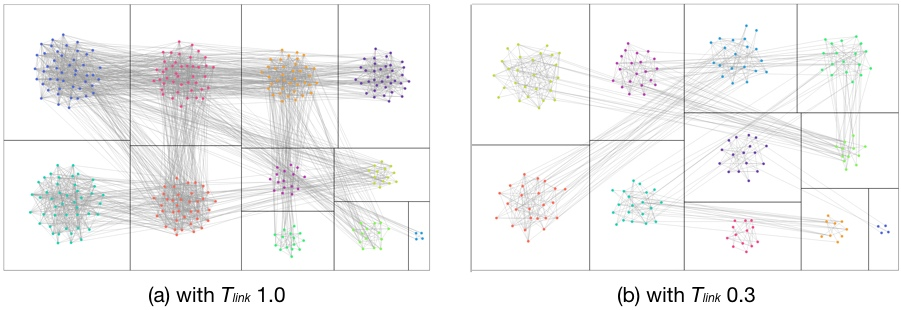
\includegraphics[width=0.7\textwidth]{tlink.jpeg}
%     \caption{Examples of our target graphs with two $T_{link}$s}
%     \label{fig:para-comp}
%     \end{center}
%     \label{左側の表へのラベル}
% \end{figure}
%
% Additionally, we implemented the same calculation as above with less links.
% Concretely, we multiplied a threshold 0.3 to $p_{in}, p_{bridge},$ and $p_{out}$, and we express the threshold as $T_{link}$ from here.
% If there are too many links in network visualization, some methods are often taken such as edge bundling or reducing links.
% Fig. \ref{fig:para-comp} shows the examples of our graphs with two $T_link$, and we can see the difficulty of understanding relationships with 1.0 for $T_{link}$.
%
% We generated real-like data in the same way as the section as 3.1, and we also set the variables link based on the calibration in 3.1, $p_{group} = 0.2$ and $p_{out} = 0.002$ .
% We chose these parameters such that we could make the elements in our data closer to real data used by Chaturvedi's, such as the number of groups, nodes, links and group size.
% In section 3 we have done experiments of two patterns, with more links and less links, and we found it difficult to solve the tasks of 4.1 with 1.0 for $T_{link}$.
% There are too many links to recognize each relationship in Fig. \ref{fig:para-comp2} (a), so we use the link-reduced data for this experiment with $T_link$ is 0.3.
% By this operation, we could utilize more readable and practical GIB networks.
% We provided all participants with the same data set and Table 2 shows the result of the same computation against the data for this experiment as the previous experiment.


After we generated data, we applied the 4 layouts to them respectively.
We can get the arrangement of tiles in this process.
The target 4 layouts arrange only boxes so we have to decide the coordinates of nodes in a box.
Though there are many ways to place nodes in boxes, we take force layout.
This method is widely used in graph drawing, where the nodes are subject to repulsive between-node forces, attractive forces between adjacent nodes and their center of gravity, and gravity from the center of the group tile to which they belong.

Also we use straight lines for edges.
Other than straight lines, we have options like edge bundling, but we wanted to calculate the total number of edge crossing which affect on the readability of graph drawing as mentioned in 3.3, so we selected the straight line.

\subsection{Experiment Design}
There are 30 questions at each task and layout respectively, so one task has 120 questions, and in total the experiment has 480 trials.
If the task changes every trial, we expect participants get confused, so participants did the same task continuously until the task ends.
Also if we show network diagrams made of the same data, participants will get accustomed to this specific data so we did not show all data repeatedly.
We generated 120 data for each task based on section 4.3, and in total we had 480 data.
We randomized the order of questions each task, so the layout of the network shown for participants were changeable every trial.
The order of task were also randomized to mitigate the effect of learning and fatigue.
Participants take a brief break at every 20 questions about a half of a minute, and take longer break at 1 task, 120 questions.
The longer break takes up to 5 minutes, and after this break we re-checked the eye-track calibration.
%
% The tasks were displayed with browser and the system was based on D3.js (https://d3js.org/).
% Nodes in the same group are colored with the same color, and we used d3.interpolateSinebow as the color variation of each group because it seems to have many colors.
We empirically set the color as gray and width of edges, as shown in figure \ref{GIB-examples}.

\subsection{Study Procedure}

We used a repeated-measures study design, and the variables of interest are:

\begin{itemize}
\item {\bf Layout of network diagram:} We utilize four kinds of GIB variants, ST-GIB, CD-GIB, FD-GIB and TR-GIB.
\item {\bf Task:} We perform 4 tasks described in section 5.1.
\end{itemize}

Participants were asked their age, gender and field of study in advance.
Next they read a manual about biometric measuring, eye-tracking and each layout of GIB.
Then we explained this experiment more in detail, followed by the tutorial step to check if they could interpret the networks and solve our tasks.
The data of trials of the tutorial are different from the actual experiment and it provided a practical procedure of the experiment.

When participants finish the all steps above, they go on to the actual experiments.
They worked on the 4 tasks in the random order to compensate for leaning and fatigue effects, and continuous 120 trials were the same task.
In terms of task 2 and 3, we asked participants two question that maximum or minimum, so early 60 trials demanded maximum one and last 60 trials were for minimum, where trials are permuted so that each half have 15 networks for each layouts respectively in these tasks.

There was no time limitation for the tasks, and the answers were sent to our server.
The participants were instructed to put emphasis on answering correctly.
If the participants put emphasis on fast solutions, higher error rates and more chaotic gaze trajectories are expected, which was not intention of this study.
Participants chose the solution by click and confirmed by pressing keyboard.

This experiment with eye tracking was conducted in a room artificially illuminated and with minimum things.
The mobile phones of participants were switched off to reduce distractions during the experiment.
The eye movements were recorded by a Tobii Pro X3-120 eye tracking system with a ASUS screen resolution of 2018 × 1920 pixels. Participants sat in front of the display with a distance of 65 cm. For the analysis software of the eye tracker, we utilized I-VT filter to discriminate if a gaze is a fixation or a saccade described in \cite{tobii}. 

\subsection{Participants}

We set a within-subjects study design with 20 participants.
All participants were Japanese, and eight of them were female and 12 were male.
Their average age was 20.8 years, and the youngest participant was at the age of 18 and the oldest at the age of 24 years.
The participants were students of our university.
Four of the participants were students of engineering, the other participants were mostly students with various majors.
All participants had normal or corrected-to-normal color vision.
The participants were compensated with 3,000 yen.
The experiments took between 1.5 to 2 hours, including the explanation and brakes. 

\section{Experimental Results}

\subsection{Generated Layouts}

There are some metrics known to influence the readability of graph drawing. We computed three measures to get insights about the user study, the number of edge crossings, the ratio of screen space wasted, and mean group aspect ratio.
% A similar evaluation is implemented by Chaturvedi et al. in \cite{chatu}.
% However, this work take only 309 data, not enough for robust evaluation.
% Also the links between groups are bundled so we can not see the relationships of nodes in different groups, which is essential for practical analysis with network graph.
% We carried out more robust evaluation by using random data based on real data and not bundled edges intended to enable to discriminate 2134 inter-links.
These 3 metrics are chosen according to the comparison of Chaturvedi's \cite{chatu} though we used edge crossings in spite of their edge-box overlap.
% They count edge-box overlap in addition to screen space wasted and mean group-box aspect ratio.
% They adopt edge-box overlaps as a measure of discernibility as several overlapping lines can make it difficult to interpret \cite{pur97,pur98,pca,becker}, but this is not fundamental because an crossing of an edge and a box does not necessarily mean an overlaps of a couple of edges.
% We decided to use the number of edge crossings instead of edge-box overlap.
We describe these metrics in detail below.

\begin{itemize}
\item {\bf Edge Crossing}

This metric can reduce the readability of graph drawing and this metric should be small.
Especially, a long inter-edge can overlaps with many other inter-edges and intra-edges of boxes on the edge's way.
We apply same layout force-directed to all boxes so we can measure how many interrupting factor are there under our data generation in 3.3.
% The number of Edge crossing is defined as
% \begin{center}
% Edge crossing = $\sum_{e_1 \in E} \sum_{e_2 \in E} overlap(e_1, e_2) $
% \end{center}
% where $E$ is the set of edges, $e_1 \neq e_2$ and the function $overlap$ takes a value of 1 only when these edges are crossing and otherwise 0.
% Total combination of $e_1$ and $e_2$ is $_n C_2$ where $n$ is the number of links.


\item {\bf Screen Space Wasted}

A 2-d screen space filling layout has the potential to be comprehensible \cite{shn92}.
In GIB, more Screen space efficiency leads boxes to become bigger and draw each network with more screen space.
When screen space is limited, a link can be too short to interpret and networks can not become aesthetic.
Screen space should not be wasted for effective visualization.
% Screen space wasted is defined as
% \begin{center}
% Percent Screen Space Wasted $= 1 - \frac{ \sum_{g \in G} area(g) }{Screen Size} $
% \end{center}
% where G is the set of groups, screen size is the area of whole screen and area(g) is the are occupied by group g.


\item {\bf Mean Group-Box Aspect Ratio}

Bruls et al. lay emphasis on that more square-like rectangles has several advantages such as screen efficiency, easiness of comparison of the size of boxes and accuracy of presentation \cite{bruls}.
They also describe that thin rectangles give rise to aliasing errors while square items are easier to detect and point at.
As we use force-directed layouts which depends on the gravity from the center of the box, the nodes in the network tends to be arranges as a shape of a sphere, so good aspect ratio, close to 1.0, is demanded.
% This ratio is described as
% \begin{center}
% Mean Group-Box Aspect Ratio $= \frac{\sum_{i=1}^{N} a_i}{N} $
% \end{center}
% where $a_i$ is aspect ratio of the $i$th group and N is the total number of groups.
\end{itemize}

\begin{table}[htb]
  \begin{center}
    \begin{tabular}{|c||c|c|c|} \hline
      Layout & edge crossing & screen space wasted & man aspect ratio \\ \hline \hline
      ST-GIB & 12536 (10496) & 0.0 (0.0) & 1.40\% (0.10) \\ \hline
      CD-GIB & 13383(11424) & 0.123 (0.073) & 2.01\% (0.40)\\ \hline
      FD-GIB & 12808 (11140) & 0.697 (0.051) & 1.0\% (0.0)\\ \hline
      TR-GIB & 11381 (9797) & 0.0 (0.0) & 1.40\% (0.10)\\ \hline
    \end{tabular}
  \end{center}
  \caption{Computation result: mean (standard deviation)}
  \label{comp-result}
\end{table}

Table \ref{comp-result} shows the result of this calculation.
In graph drawing we demand less edge overlaps, low aspect ratio, and small screen space wasted.

As a result, we can observe that TR-GIB had the least edge crossings than the others as shown in Table \ref{comp-result}, which indicates that TR-GIB is the most effective for reducing edge overlaps.
% The case with the same number of groups and less links means that there are few inter links, which is not practical and out of the purposes of some layouts that aim to express relationships between groups, so we should suppose a condition with inter-links to some extent when we compare the capabilities to reduce edge crossings, where TR-GIB had the advantage of the others.
% This tendency could be observed both of when there are many links ($T_{link}$ is 1.0) and not ($T_{link}$ is 0.3).

In terms of the ratio of screen space wasted, it was good at ST-GIB and TR-GIB, followed by CD-GIB as we can see in Table \ref{comp-result}.
It also represent that FD-GIB had the best aspect-ratio, followed by ST-GIB and TR-GIB.
ST-GIB and TR-GIB were good at both of space efficiency and aspect, and CD-GIB and FD-GIB were good at only either of them.

% <<<<<<< HEAD
% =======
% %
% \section{User Study Experiments}
% %

% In addition to computational experiment, we also worked on the user study experiment with eye-track system. We intended to reveal which layout were superior in some tasks through user study. The layouts of GIB we compared were the same as section 3, STGIB, CDGIB, FDGIB and TRGIB. In addition to accuracy and completion time of tasks, we also measured eye-tracking data to evaluate layouts quantitatively. By using eye-track system, we can give elaborates discussion on the result \cite{eyemethod}. We describe this experiment in this section.

% \subsection{Task}
% For the first thing of user study, we first set up our tasks according to Vehlow et al. \cite{survey} and Saket et al. \cite{saket}. Vehlow et al. introduces 4 kinds of task taxonomy about evaluation of clustered graph visualization, Group-only task (GOT), group-vertex Task (GVT), group-edge task (GET) and group-network task (GNT). Among these tasks, GOT, GVT and GNT tasks can be applied for our GIB evaluation because GET task is for networks which its edges are grouped. Saket et al. also provides 4 kinds of task. There are Group Only Tasks, Group-Node Tasks, Group-Link Tasks, Group-Network Tasks and all of them can be applied to ours, but we saw that Vehlow's GNT include Saket's Group-Node Tasks and Group-Network Tasks. Vehlow et al. and Saket et al. are also describing examples of each kind of tasks. For instance of the Group-Node Tasks, there are a task of finding the group with the maximum number of nodes. We selected our task from these examples, and we imposed on the participants the following 4 task.
% >>>>>>> b724c83bc91598189dc81dfa000b3821b03effd8

\subsection{Task Results}

In this section we describe the result of the user study experiment, not including the eye-track data discussed in the following section.
The result of user study is shown in table \ref{user-result} We conducted one-way ANOVA, 4 layouts against each task, where $p$ was $0.05$ against the accuracy and the task completion time as represented at table \ref{anova}.
We adopt one-way ANOVA based on an idea that each layout has its advantages and disadvantages and all tasks are independent.
% =======
% \subsection{Experimental Design}
% We used a repeated-measures study design, and the variables of interest are:

% \begin{itemize}
% \item {\bf Layout of network diagram:} We utilize four kinds of GIB layouts, ST-GIB, CD-GIB, FD-GIB and TR-GIB.
% \item {\bf Task:} We perform 4 tasks described in section 5.1.
% \end{itemize}

% There are 30 questions at each task and layout respectively, so one task has 120 questions, and in total the experiment has 480 trials. If the task changes every trial, we expect participants get confused, so participants did the same task continuously until the task ends. Also if we show network diagrams made of the same data, participants will get accustomed to this specific data so we did not show all data repeatedly. We generated 120 data for each task based on section 4.3, and in total we had 480 data. We randomized the order of questions each task, so the layout of the network shown for participants were changeable every trial. The order of task were also randomized to mitigate the effect of learning and fatigue. Participants take a brief break at every 20 questions about a half of a minute, and take longer break at 1 task, 120 questions. The longer break takes up to 5 minutes, and after this break we re-checked the eye-track calibration. 

% \subsection{Environment and Technical Setup}
% This experiment with eye tracking was conducted in a room artificially illuminated and with minimum things. The mobile phones of participants were switched off to reduce distractions during the experiment. The eye movements were recorded by a Tobii Pro X3-120 eye tracking system with a ASUS screen resolution of 2018 × 1920 pixels. Participants sat in front of the display with a distance of 65 cm. For the analysis software of the eye tracker, we utilized I-VT filter to discriminate if a gaze is a fixation or a saccade described in \cite{tobii}. 

% The tasks were displayed with browser and the system was based on D3.js (https://d3js.org/). Nodes in the same group are colored with the same color, and we used d3.interpolateSinebow as the color variation of each group because it seems to have many colors. We empirically set the color as gray and width of edges, as shown in figure 1.

% \subsection{Participants}
% We set a within-subjects study design with 20 participants. All participants were Japanese, and eight of them were female and 12 were male. Their average age was 20.8 years, and the youngest participant was at the age of 18 and the oldest at the age of 24 years. The participants were students of our university. Four of the participants were students of engineering, the other participants were mostly students with various majors. All participants had normal or corrected-to-normal color vision. The participants were compensated with 3,000 yen. The experiments took between 1.5 to 2 hours, including the explanation and brakes.

% \subsection{Study Procedure}
% Participants were asked their age, gender and field of study in advance. Next they read a manual about biometric measuring, eye-tracking and each layout of GIB. Then we explained this experiment more in detail, followed by the tutorial step to check if they could interpret the networks and solve our tasks. The data of trials of the tutorial are different from the actual experiment and it provided a practical procedure of the experiment.

% When participants finish the all steps above, they go on to the actual experiments. They worked on the 4 tasks in the random order to compensate for leaning and fatigue effects, and continuous 120 trials were the same task. In terms of task 2 and 3, we asked participants two question that maximum or minimum, so early 60 trials demanded maximum one and last 60 trials were for minimum, where trials are permuted so that each half have 15 networks for each layouts respectively in these tasks.

% There was no time limitation for the tasks, and the answers were sent to our server. The participants were instructed to put emphasis on answering correctly. If the participants put emphasis on fast solutions, higher error rates and more chaotic gaze trajectories are expected, which was not intention of this study. Participants chose the solution by click and confirmed by pressing keyboard.

% \subsection{result}

% In this section we describe the result of the user study experiment, not including the eye-track data discussed in the following section. The result of user study is shown in table 3 We conducted one-way ANOVA, 4 layouts against each task, where $p$ was $0.05$ against the accuracy and the task completion time as represented at table 4. We adopt one-way ANOVA based on an idea that each layout has its merits and demerits and all tasks are independent.
% >>>>>>> b724c83bc91598189dc81dfa000b3821b03effd8

\begin{table}[htb]
  \begin{center}
    \begin{tabular}{|c||c|c|c|c|} \hline
      Layout & task1 & task2 & task3 & task4 \\ \hline \hline
      ST-GIB & 98.1\% (3.987s) & 89.6\% (2.535s) & 67.4\% (3.606s) & 62.8\% (5.387s) \\ \hline
      CD-GIB & 98.2\% (4.527s) & 76.9\% (2.761s) & 67.2\% (3.843s) & 59.3\% (5.588s)\\ \hline
      FD-GIB & 96.7\% (4.919s) & 82.9\% (2.427s) & 78.8\% (3.382s) & 59.3\% (5.518s)\\ \hline
      TR-GIB & 98.1\% (4.493s) & 83.6\% (2.713s) & 72.8\% (3.845s) & 63.5\% (5.128s)\\ \hline
    \end{tabular}
  \end{center}
   \caption{Result of user study: mean accuracy (mean completion time)}
  \label{user-result}
\end{table}

At task 1, we can see a significant difference in task completion time, and ST-GIB is superior to the others, and FD-GIB is the worst.
Participants could count the number of groups faster in ST-GIB, and this is against the hypothesis 1.
FD-GIB needed the longest time to recognize the answer.

There are significant difference at both of the accuracy and the time in task 2.
Participants had the highest accuracy in ST-GIB, and the lowest in CD-GIB.
In terms of task completion time, FD-GIB was the best.
The hypothesis 2 is refuted, and the hypothesis 3 could be confirmed.


FD-GIB got the highest score at both of accuracy and time in task 3, and we can also see significant differences among them, and this refute the hypothesis 5.
The hypothesis 4 could confirmed as TR-GIB got the second highest accuracy.

In task4, there were no significant differences in accuracy and time, so the hypothesis 6 could not be confirmed.

\begin{table}[h]
  \begin{center}
    \begin{tabular}{|c||c|c|c|c|} \hline
      & task1 & task2 & task3 & task4 \\ \hline \hline
        Accuracy & 0.2377 & 2.579e-7 & 1.303e-5 & 0.3039 \\ \hline
        Time & 9.009e-16 & 7.571e-5 & 4.706e-5 & 0.06275\\ \hline
    \end{tabular}
  \end{center}
  \caption{P-value of ANOVA for the accuracy and completion time}
  \label{anova}
\end{table}

\subsection{Eye tracking Results}

We collected eye tracking data during user study and analyzed it based on \cite{eyemethod}, where Andrienko el al. describes the visual analytics methodology against tasks and gives as guidelines for method selection. 
We selected trajectory maps as shown in Fig. \ref{traje}, which were useful to grasp the overall spatial pattern of movements, but sometimes not effective when there are so many data.
However our eye-track data for graphs are not enormous, of 20 participants, so we selected trajectory maps in order to see participants' eye-movements.
We also computed total count of gazes in Table \ref{time-CV}. We can see the count of gazes are strongly connected to the task completion time shown in Table \ref{user-result}. According to Pearson's correlation analysis, there is a strong relationships ($r = 0.993, p = 1.65 \mathrm{e}{-14}$.

\begin{figure}[h]
  \def\@captype{table}
  \begin{minipage}[c]{.48\textwidth}
  	\begin{center}
    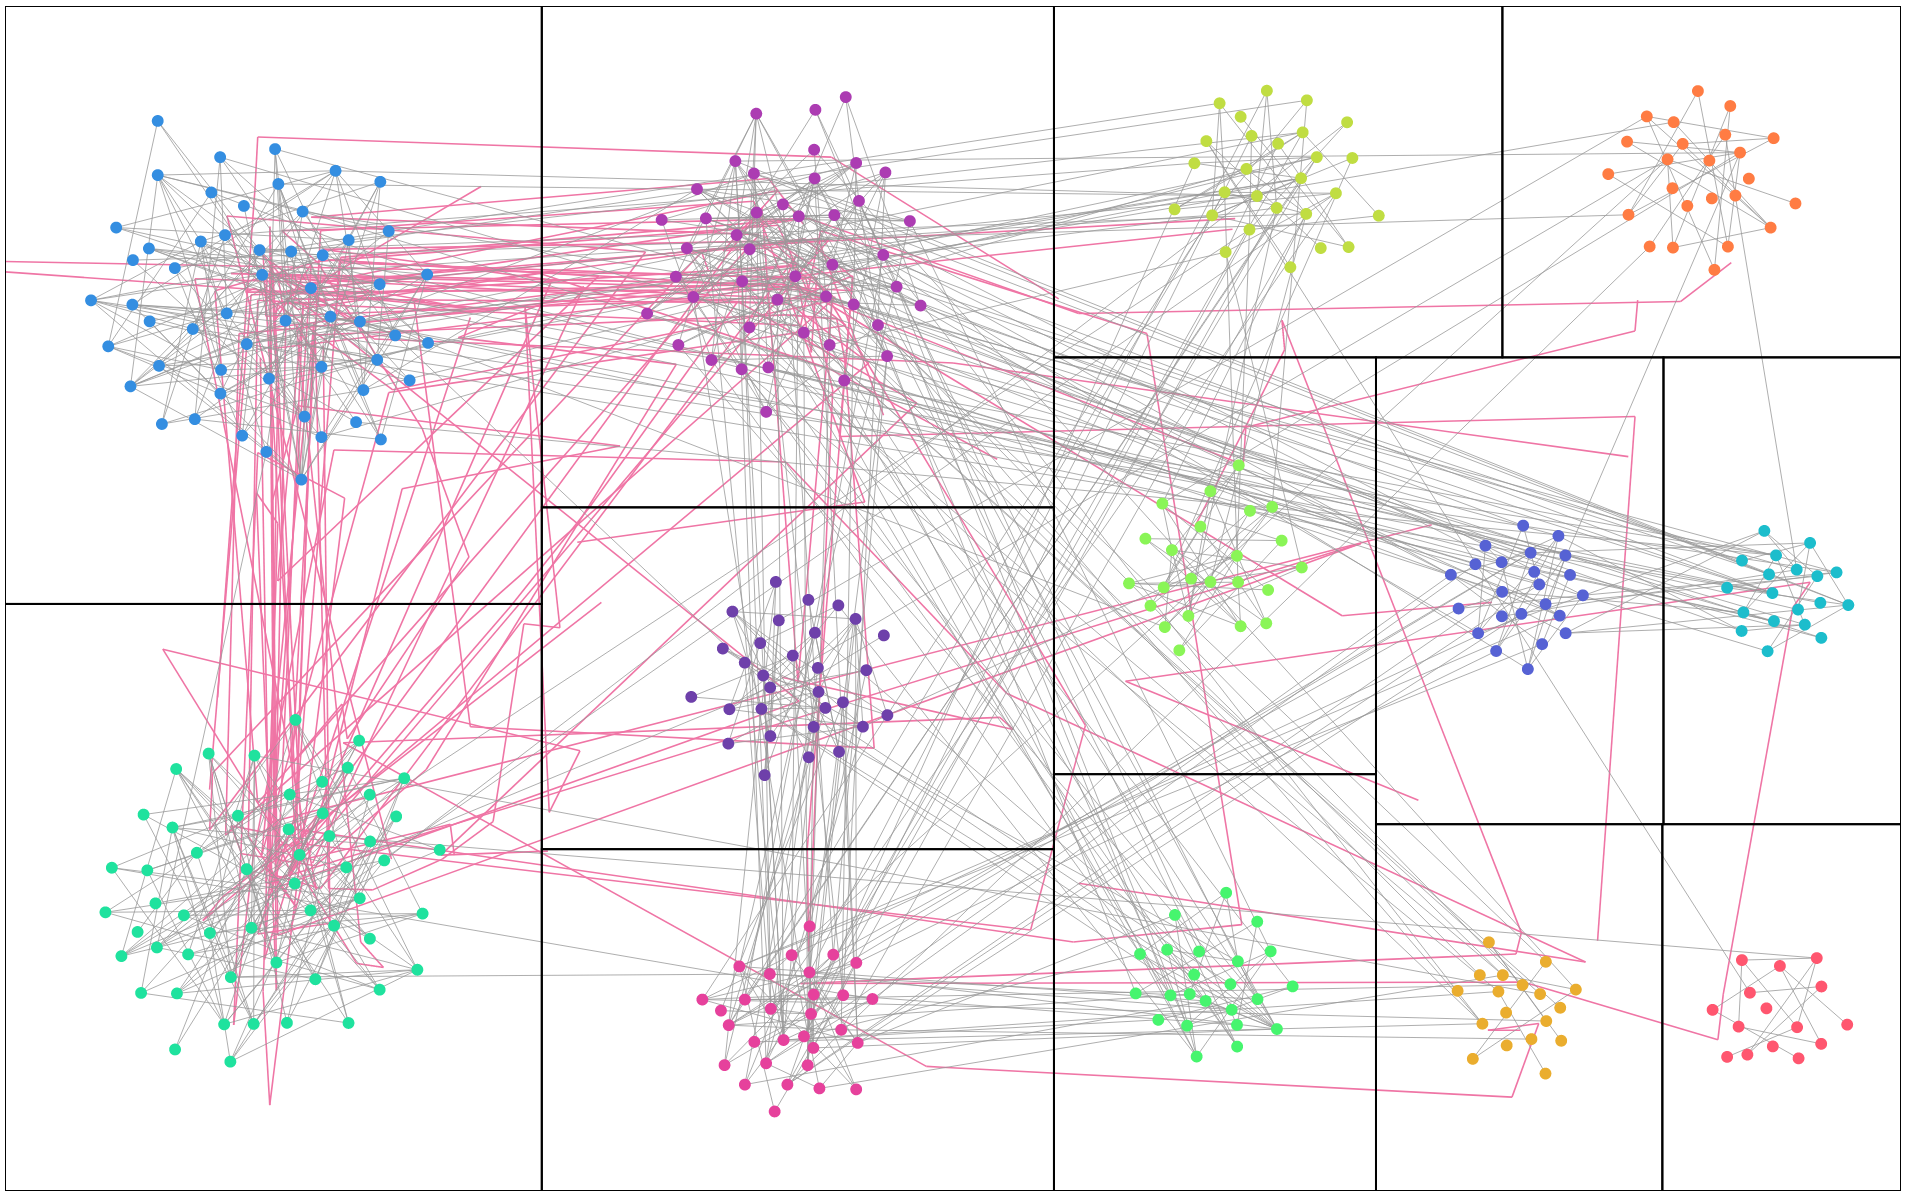
\includegraphics[width=1.0\textwidth]{4-3.png}
    \caption{An example of trajectory map: pink lines represent the gaze trajectories.}
    \end{center}
    \label{traje}
  \end{minipage}
  %
  \hfill
  %
  \begin{minipage}[c]{.48\textwidth}
  \begin{center}
      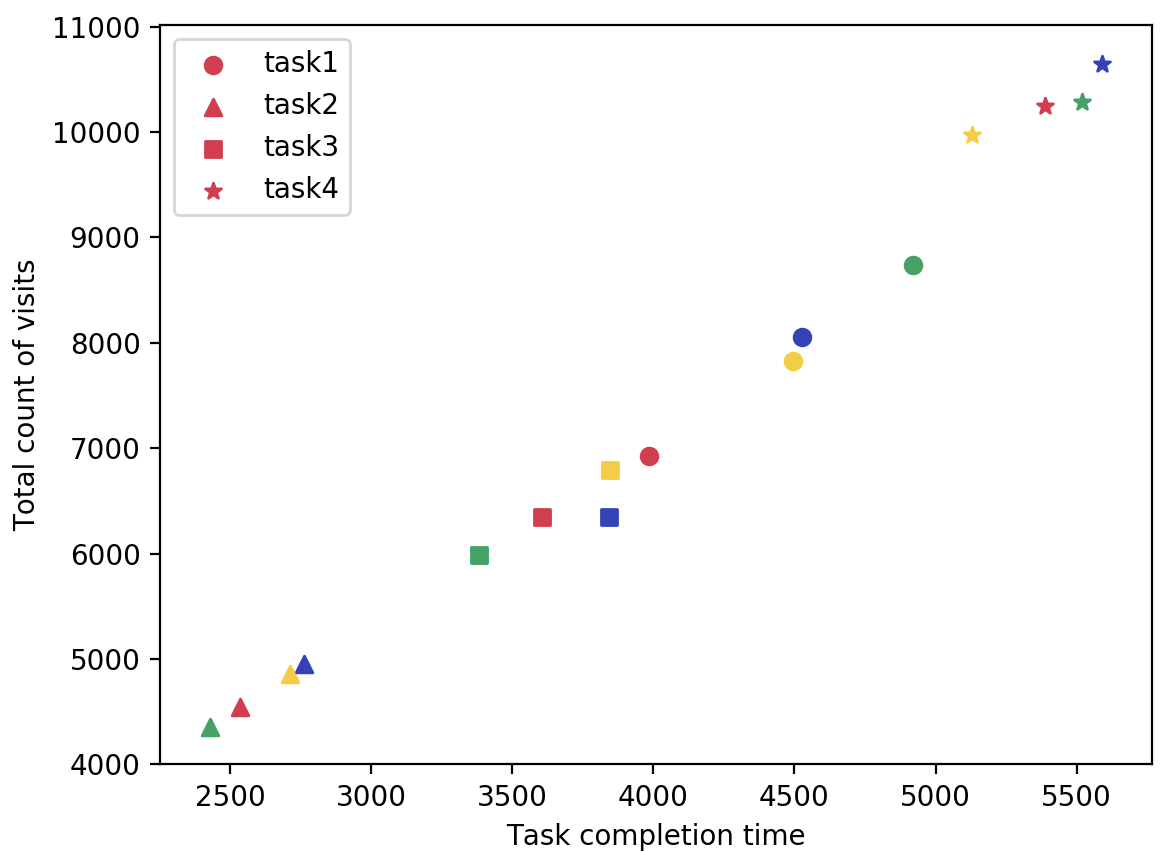
\includegraphics[width=0.8\textwidth]{time-count.png}
        \caption{The relationships between task completion time and total count of visits, where ST-GIB is red, CD-GIB is blue, FD-GIB is green, and TR-GIB is yellow.}
    \end{center}
    \label{time-CV}
  \end{minipage}
\end{figure}

\section{Discussion}
From here we discuss the result above using the eye-track data.
By using eye-track system, we aimed to clarify the reason why a layout is better or not than the others.

In FD-GIB participants could not catch the answer as early as the others in task 1, where we observed that the trajectories of gazes are prevailed all over the boxes in all layouts though the space occupied by boxes is small in FD-GIB.
The total count of visits shows a clue of the reason of the difference, many visits.
Participant took many visits in FD-GIB to count the number of groups, which indicates that FD-GIB takes much time to count the number of groups and supports the result.
We suppose that many visits is caused by re-counting of participants, which means the difficulty to count in FD-GIB mainly because of space wasting.

In task 2, ST-GIB had the highest accuracy and the lowest is CD-GIB.
The layout with the best aspect ratio, FD-GIB, is not as accurate as ST-GIB and TR-GIB, so we can say ST-GIB and TR-GIB has good aspect enough to understand its box's size.
The reason why ST-GIB got the highest accuracy in this task is, we suppose, that the layout arranges the boxes in the order of their sizes actually in our algorithm.

CD-GIB and TR-GIB had many visits of gazes and this may caused the slowness of task completion like task 1, but this can not be guess as the factor of the difference of accuracy because TR-GIB had relatively high accuracy.
By observing trajectory maps, we guess this was caused by more dispersed gaze in CD-GIB.
In CD-GIB, in addition to the not good aspect ratio, boxes with similar areas can be arranged with far distance among them, while ST-GIB variants big boxes close to each other, which is expected to make it easy to compare their sizes.
The bad aspect ratio and dispersed boxes might confuse participants and increase the total visits.

FD-GIB was the best at both of accuracy and completion time in task 3, and the TR-GIB had the second highest accuracy.
This result corresponds with that of computation at 4.1 that the number of edge crossing were small in FD-GIB and TR-GIB, which interrupt the readability \cite{becker,pur97,pur98,pca}.

As a result of analyzing the trajectory map, we found that the main strategy in task 3 was comparing some large or small boxes.
A bigger/smaller box tend to have more/less links, so participants extracted some big or small boxes along the task for the first step, followed by the next step of comparison of links in the boxes, where FD-GIB seems to have outperformed the TR-GIB because the accuracies of task 2, a similar process of extraction in this task, were almost the same.
The reason why FD-GIB was easier than TR-GIB though that has more edge-crossings is supposed to the size of the box.
Our task required only a box with the most or the least links, so participants could discriminate the answer by only see the dense of links as depth of color.
In our graphs, the part with many links looks dark and less are white because of the color of links, gray.
We suppose that it is easier to discern the part with dark or pale color in FD-GIB, which have smaller boxes.
When another task to see intra-links is used such as finding the vertex with the highest degree, TR-GIB can be effective because its bigger boxes can show each relationships clearly.

In task4, there are no significant difference although the number of edge overlaps are different.
The gaze trajectories were observed along the inter-edges (shown in Appendix).
We reckon that undesirable long inter-edges make it easier to to find the answer in this task contrary to our hypothesis 7, which produce edge crossings.
The long edges stands out visually so the box with many and long edges can be detect easily.

After all, FD-GIB and TR-GIB made good achievements in our tasks, while CD-GIB was not good at all tasks.
ST-GIB was not bad in task 1, task2 and task3 though it does not consider the relationships between groups.
Task 3 make difference between FD-GIB and TR-GIB which have different size of its box, so we recommend to choose either of these two layouts properly for the purpose of users.


%
\section{Conclusions and Future Work}
%

In this study, we worked on the evaluation of 4 GIB layouts by user study with eye tracking. We find out which layout is better than the other and we got some evidences about the result.

Our computation gives us the superiorities of FD-GIB, with good aspect and edge cross, and TR-GIB, with good aspect to some extent and edge crossings.
Also the user study experiment tells us their higher performances.
ST-GIB was good at understanding the size of each box, but not at interpreting links.
We revealed that FD-GIB and TR-GIB are effective but they have their advantages and disadvantages.
FD-GIB is strong at showing the number of links, a blurred information, but TRGIB is expected stronger at representing more concrete relationships such as a link connection between specific two nodes.

For the limitations of this work, other algorithms or methods can be taken to generate random data, though we aimed to make it realistic.
Especially, used only one set of parameters in user study so other cases are interesting.
Besides that, there are many other ways of expressing nodes and edges and arranging nodes which may influence the results.
We found that undesirable long edges were effective in task 4, hence another task may leads us to further results.

Our massive eye-track data can be take further analysis for the future work.
There are so many methods to cope with eye-track data which we have not done in this study, which may give us a novel discovery.
Moreover, we are now preparing a web-based visualizing system of GIB in public.
We hope that anyone can avail GIB variants easily and make new findings with these layouts.

\newpage

%
% ---- Bibliography ----
%
\begin{thebibliography}{5}
%

\bibitem{survey}
Corinna Vehlow, Fabian Beck, and Daniel Weiskopf. 2017. Visualizing Group Structures in Graphs: A Survey. Comput. Graph. Forum 36, 6 (September 2017), 201-225. DOI: https://doi.org/10.1111/cgf.12872

\bibitem{saket}
Saket, Bahador, Paolo Simonetto, and Stephen Kobourov. "Group-level graph visualization taxonomy." arXiv preprint arXiv:1403.7421 (2014)

\bibitem{bruls}
Bruls, Mark, Kees Huizing, and Jarke J. Van Wijk. "Squarified treemaps." Data visualization 2000. Springer, Vienna, 2000. 33-42.

\bibitem{rodri}
E. M. Rodrigues, N. Milic-Frayling, M. Smith, B. Shneiderman and D. Hansen, "Group-in-a-Box Layout for Multi-faceted Analysis of Communities," 2011 IEEE Third International Conference on Privacy, Security, Risk and Trust and 2011 IEEE Third International Conference on Social Computing, Boston, MA, 2011, pp. 354-361.
doi: 10.1109/PASSAT/SocialCom.2011.139

\bibitem{chatu}
Chaturvedi, Snigdha, et al. "Group‐in‐a‐Box Meta‐Layouts for Topological Clusters and Attribute‐Based Groups: Space‐Efficient Visualizations of Network Communities and Their Ties." Computer Graphics Forum. Vol. 33. No. 8. 2014.

\bibitem{gansner}
Gansner, Emden R., and Yifan Hu. "Efficient node overlap removal using a proximity stress model." International Symposium on Graph Drawing. Springer, Berlin, Heidelberg, 2008.

\bibitem{harel}
Harel, David, and Yehuda Koren. "Graph drawing by high-dimensional embedding." International symposium on graph drawing. Springer, Berlin, Heidelberg, 2002.

\bibitem{koren}
Koren, Yehuda, Liran Carmel, and David Harel. "Drawing huge graphs by algebraic multigrid optimization." Multiscale Modeling \& Simulation 1.4 (2003): 645-673.

\bibitem{hachul1}
Hachul, Stefan, and Michael Jünger. "An experimental comparison of fast algorithms for drawing general large graphs." International Symposium on Graph Drawing. Springer, Berlin, Heidelberg, 2005.

\bibitem{hachul2}
Hachul, Stefan, and Michael Jünger. "Large-Graph Layout Algorithms at Work: An Experimental Study." J. Graph Algorithms Appl. 11.2 (2007): 345-369.

\bibitem{becker}
Becker, Richard A., Stephen G. Eick, and Allan R. Wilks. "Visualizing network data." IEEE Transactions on visualization and computer graphics 1.1 (1995): 16-28.

\bibitem{shn92}
Shneiderman, Ben. "Tree visualization with tree-maps: 2-d space-filling approach." ACM Transactions on graphics (TOG) 11.1 (1992): 92-99.

\bibitem{onoue}
Onoue, Yosuke, and Koji Koyamada. "Optimal tree reordering for group-in-a-box graph layouts." SIGGRAPH Asia 2017 Symposium on Visualization. ACM, 2017.

\bibitem{kaufman}
Kaufmann, Michael, and Dorothea Wagner. "Drawing graphs: methods and models, volume 2025 of Lecture Notes in Computer Science." (2001).

\bibitem{tamassia}
Tamassia, Roberto, ed. Handbook of graph drawing and visualization. CRC press, 2013.

\bibitem{newman10}
Newman, Mark. Networks: an introduction. Oxford university press, 2010.

\bibitem{newman04}
Newman, Mark EJ. "Detecting community structure in networks." The European Physical Journal B 38.2 (2004): 321-330.

\bibitem{newman02}
Girvan, Michelle, and Mark EJ Newman. "Community structure in social and biological networks." Proceedings of the national academy of sciences 99.12 (2002): 7821-7826.

\bibitem{newman06}
Newman, Mark EJ. "Modularity and community structure in networks." Proceedings of the national academy of sciences 103.23 (2006): 8577-8582.

\bibitem{shn92}
Shneiderman, Ben. "Tree visualization with tree-maps: 2-d space-filling approach." ACM Transactions on graphics (TOG) 11.1 (1992): 92-99.

\bibitem{burchtree}
Burch, Michael, et al. "Evaluation of traditional, orthogonal, and radial tree diagrams by an eye tracking study." IEEE Transactions on Visualization and Computer Graphics 17.12 (2011): 2440-2448.

\bibitem{pur97}
Purchase, Helen. "Which aesthetic has the greatest effect on human understanding?." International Symposium on Graph Drawing. Springer, Berlin, Heidelberg, 1997.

\bibitem{pur98}
Purchase, Helen C. "Performance of layout algorithms: Comprehension, not computation." Journal of Visual Languages \& Computing 9.6 (1998): 647-657.

\bibitem{pca}
Purchase, Helen C., David Carrington, and Jo-Anne Allder. "Empirical evaluation of aesthetics-based graph layout." Empirical Software Engineering 7.3 (2002): 233-255.

\bibitem{eyemethod}
Andrienko, Gennady, et al. "Visual analytics methodology for eye movement studies." IEEE Transactions on Visualization and Computer Graphics 18.12 (2012): 2889-2898.

\bibitem{harel-koren}
Harel, David, and Yehuda Koren. "A fast multi-scale method for drawing large graphs." International symposium on graph drawing. Springer, Berlin, Heidelberg, 2000.

\bibitem{tobii}
Olsen, Anneli. "The Tobii I-VT fixation filter." Tobii Technology (2012).

\end{thebibliography}

\end{document}
